% ---------------------------------------------------------------------------
% Author guideline and sample document for EG publication using LaTeX2e input
% D.Fellner, v1.13, Jul 31, 2008

\documentclass{egpubl}
\usepackage{eurovis2018}
\Full_EuroVis
% --- for  Annual CONFERENCE
% \ConferenceSubmission   % uncomment for Conference submission
%\ConferencePaper        % uncomment for (final) Conference Paper
% \STAR                   % uncomment for STAR contribution
% \Tutorial               % uncomment for Tutorial contribution
% \ShortPresentation      % uncomment for (final) Short Conference Presentation
% \Areas                  % uncomment for Areas contribution
% \MedicalPrize           % uncomment for Medical Prize contribution
% \Education              % uncomment for Education contribution
%
% --- for  CGF Journal
% \JournalSubmission    % uncomment for submission to Computer Graphics Forum
% \JournalPaper         % uncomment for final version of Journal Paper
%
% --- for  CGF Journal: special issue
% \SpecialIssueSubmission    % uncomment for submission to Computer Graphics Forum, special issue
% \SpecialIssuePaper         % uncomment for final version of Journal Paper, special issue
%
% --- for  EG Workshop Proceedings
% \WsSubmission    % uncomment for submission to EG Workshop
% \WsPaper         % uncomment for final version of EG Workshop contribution
%
 % \electronicVersion % can be used both for the printed and electronic version
\SupplementalMaterial

% !! *please* don't change anything above
% !! unless you REALLY know what you are doing
% ------------------------------------------------------------------------

% for including postscript figures
% mind: package option 'draft' will replace PS figure by a filname within a frame
\ifpdf \usepackage[pdftex]{graphicx} \pdfcompresslevel=9
\else \usepackage[dvips]{graphicx} \fi

\PrintedOrElectronic

% prepare for electronic version of your document
\usepackage{t1enc,dfadobe}

\usepackage{egweblnk}
\usepackage{cite}
\usepackage{xspace}

% For backwards compatibility to old LaTeX type font selection.
% Uncomment if your document adheres to LaTeX2e recommendations.
% \let\rm=\rmfamily    \let\sf=\sffamily    \let\tt=\ttfamily
% \let\it=\itshape     \let\sl=\slshape     \let\sc=\scshape
% \let\bf=\bfseries

% end of prologue

% ---------------------------------------------------------------------
% EG author guidelines plus sample file for EG publication using LaTeX2e input
% D.Fellner, v1.17, Sep 23, 2010


\title[Reapplication of SetCoLa Specifications for Biological Networks]%
{
  Reapplication of SetCoLa Specifications for Biological Networks
  \vspace{-20pt}
}

% for anonymous conference submission please enter your SUBMISSION ID
% instead of the author's name (and leave the affiliation blank) !!
\author[Jane Hoffswell, Alan Borning, and Jeffrey Heer]
{
  Jane Hoffswell,
  Alan Borning,
  and Jeffrey Heer
  \\\vspace{-10pt}
  % For Computer Graphics Forum: Please use the abbreviation of your first name.
  Paul G. Allen School of Computer Science \& Engineering, University of Washington
}

% ------------------------------------------------------------------------

% if the Editors-in-Chief have given you the data, you may uncomment
% the following five lines and insert it here
%
% \volume{27}   % the volume in which the issue will be published;
% \issue{1}     % the issue number of the publication
% \pStartPage{1}      % set starting page


%-------------------------------------------------------------------------
%!TEX root = constraint-layout.tex
\usepackage{soul}
\usepackage{color}

\definecolor{red}{RGB}{178,34,34}
\definecolor{orange}{rgb}{1, 0.8, 0.4}
\definecolor{lightgreen}{RGB}{121, 210, 121}
\definecolor{lightpurple}{RGB}{153, 102, 255}
\definecolor{gray}{RGB}{166, 166, 166}

%% Note: One of the following blocks of \newcommmands should be commented in to show/hide comments
% \newcommand{\cut}[1]{}
% \newcommand{\todo}[1]{}

%% Note: Comment this in to see all comments and unfinished text in the paper.
\newcommand{\todo}[1]{\textcolor{red}{[TODO] \emph{#1}}}
\newcommand{\cut}[1]{\textcolor{red}{\st{#1}}}
\newcommand{\orange}[1]{\textcolor{orange}{#1}}
\newcommand{\green}[1]{\textcolor{lightgreen}{#1}}
\newcommand{\purple}[1]{\textcolor{lightpurple}{#1}}
\newcommand{\gray}[1]{\textcolor{gray}{#1}}

% Text colors based on the figure colors
% \definecolor{figuregreen}{RGB}{210,231,211} % light figure green
% \definecolor{figureblue}{RGB}{183,217,254} % light figure blue
% \definecolor{figurepurple}{RGB}{205,183,219} % light figure purple
% \definecolor{figuregreen}{RGB}{82,102,0} % dark figure green
% \definecolor{figureblue}{RGB}{39,66,102} % dark figure blue
% \definecolor{figurepurple}{RGB}{83,54,102} % dark figure purple
\definecolor{figuregreen}{RGB}{134,166,0} % medium figure green: brightness: 40->65
\definecolor{figureblue}{RGB}{63,108,166} % medium figure blue: brightness: 40->65
\definecolor{figurepurple}{RGB}{135,88,166} % medium figure purple: brightness 40->65
\newcommand{\figuregreen}[1]{\textcolor{figuregreen}{#1}}
\newcommand{\figureblue}[1]{\textcolor{figureblue}{#1}}
\newcommand{\figurepurple}[1]{\textcolor{figurepurple}{#1}}


\newcommand{\projectname}{SetCoLa\xspace}
\newcommand{\constraint}[1]{
  \vspace{-13px}
  \begin{flushright}
  \scriptsize
  #1
  \end{flushright}
}
\newtheorem{definition}{Definition}

\newcommand{\jheer}[1]{\textbf{JH: #1}}

\newcommand{\feedback}[2]{\purple{\textbf{#1:} #2}}

%!TEX root = constraint-layout.tex

% \newcommand{\teaserFigure}{
% 	\teaser{
% 		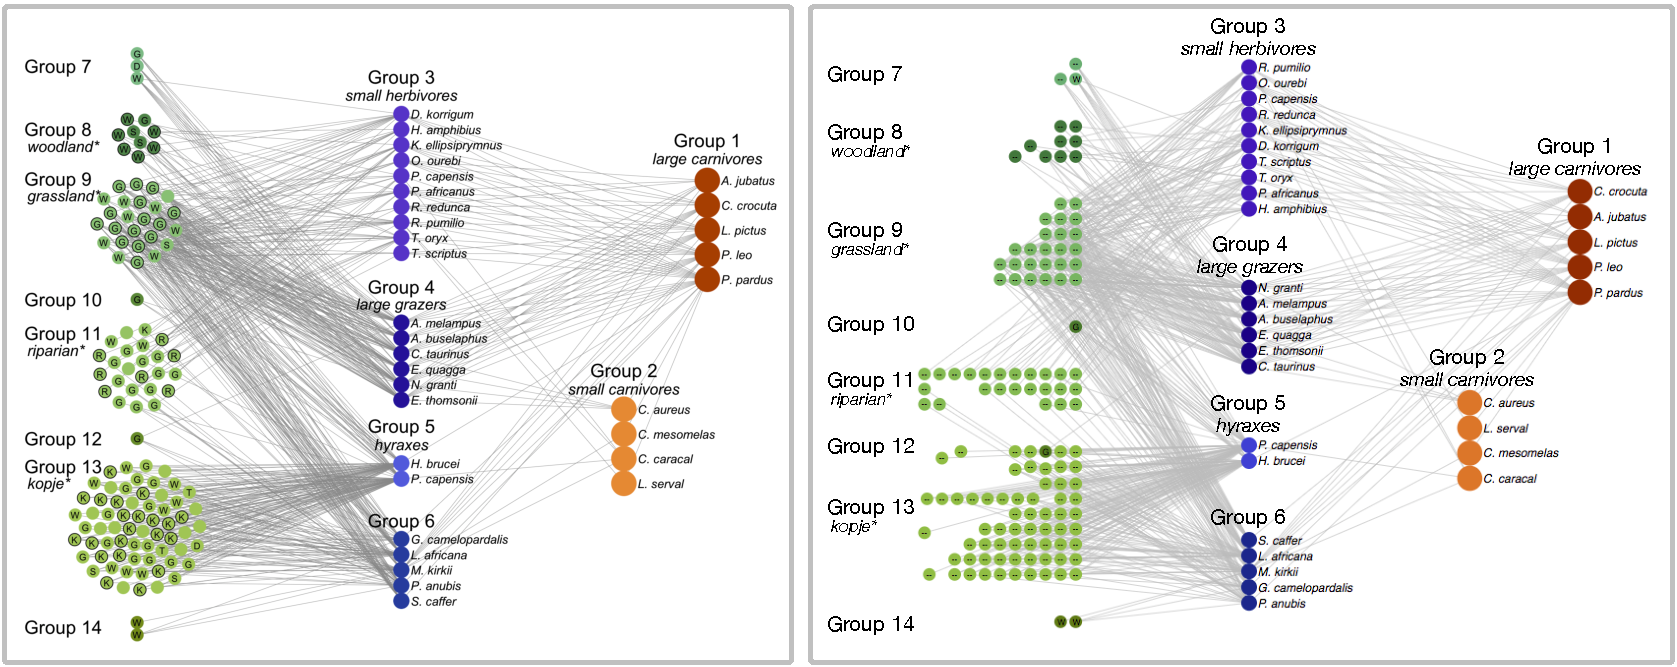
\includegraphics[width=\linewidth]{figures/serengeti-layout.pdf}
% 		\centering
% 	  \caption{\label{fig:teaser}}

% 	}
% }

\newcommand{\serengetiLayoutColumn}{
  \begin{figure}[t!]
    \centering
    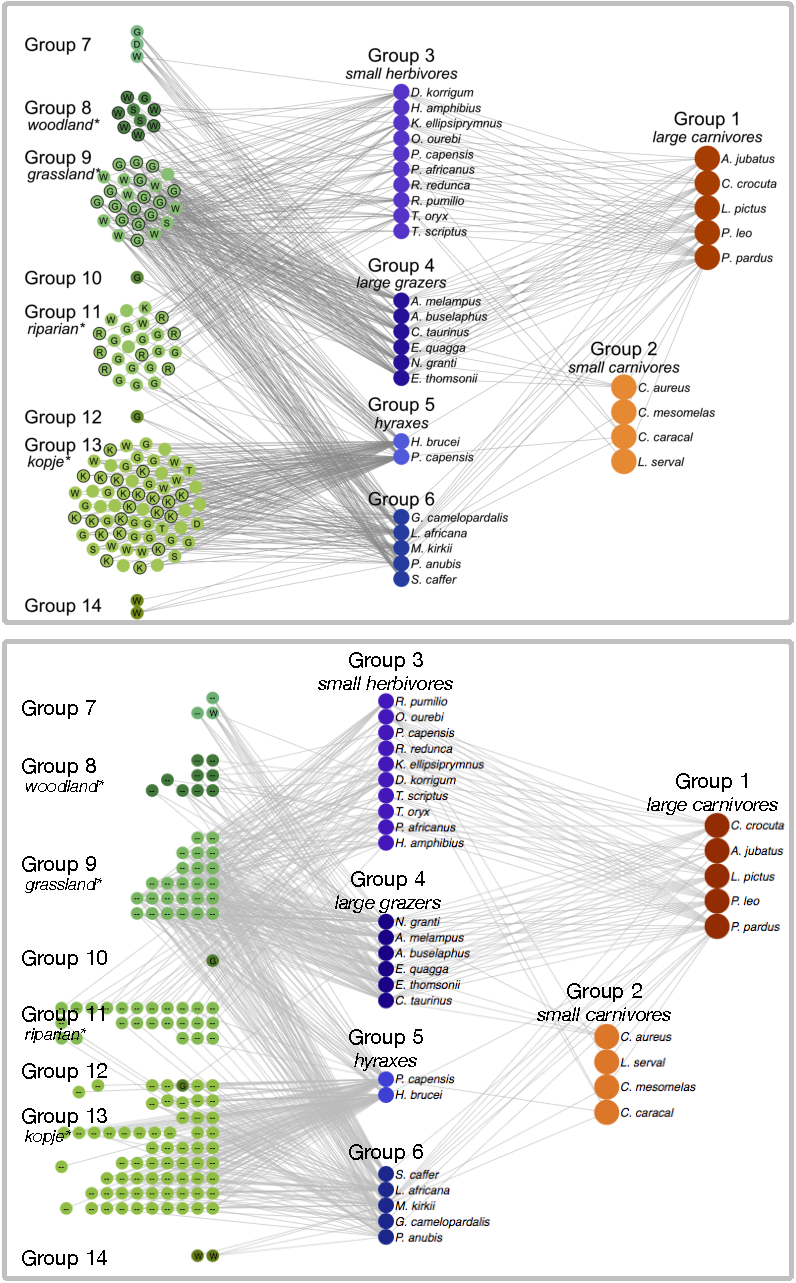
\includegraphics[width=0.81\columnwidth]{figures/serengeti-layout-column.pdf}
    {\caption{\label{fig:serengeti-layout}
    The layout for the Serengeti food web using our constraint language, as compared to Baskerville et al. \cite{baskerville2011spatial}.}}
    \vspace{-40px}
  \end{figure}
}

%%%%%%%%%%%%%%%%%%%%%%%%%%%%%%%%%%
%%%%%%%%%%%%% Design %%%%%%%%%%%%%
%%%%%%%%%%%%%%%%%%%%%%%%%%%%%%%%%%

\newcommand{\smallTreeExample}{
  \begin{figure}[t!]
    \centering
    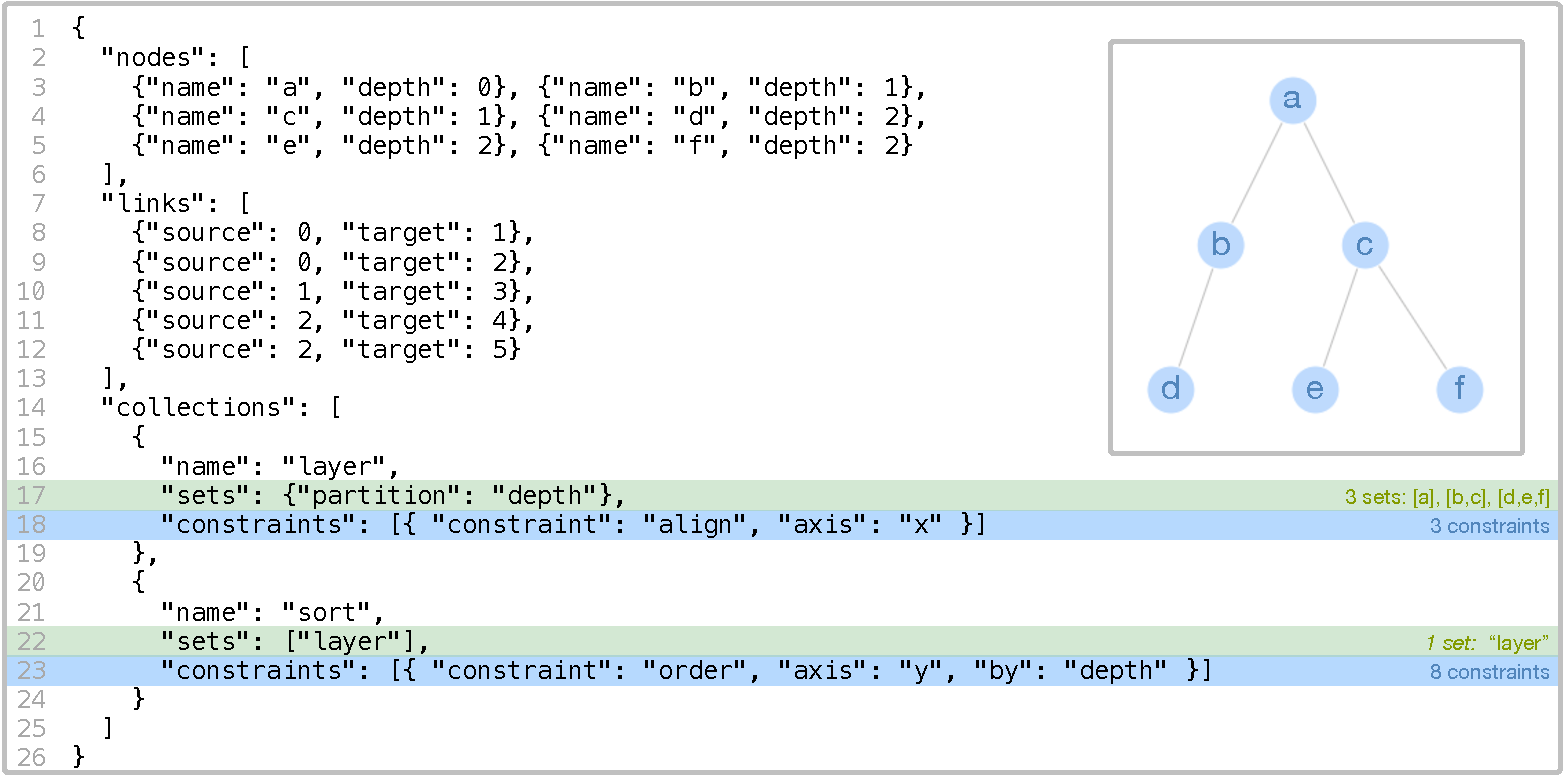
\includegraphics[width=\columnwidth]{figures/small-tree-example.pdf}
    {\caption{\label{fig:small-tree-example}
    The full \projectname\ specification for a small tree with six nodes. Nodes are split into sets based on their depth from the root \texttt{a}, and aligned. A new collection is formed containing the ``layer'' set and the layers are ordered by their depth to form the tree.
    }}
    \vspace{-20px}
  \end{figure}
}

\newcommand{\contradictionExample}{
  \begin{figure}[t!]
    \centering
    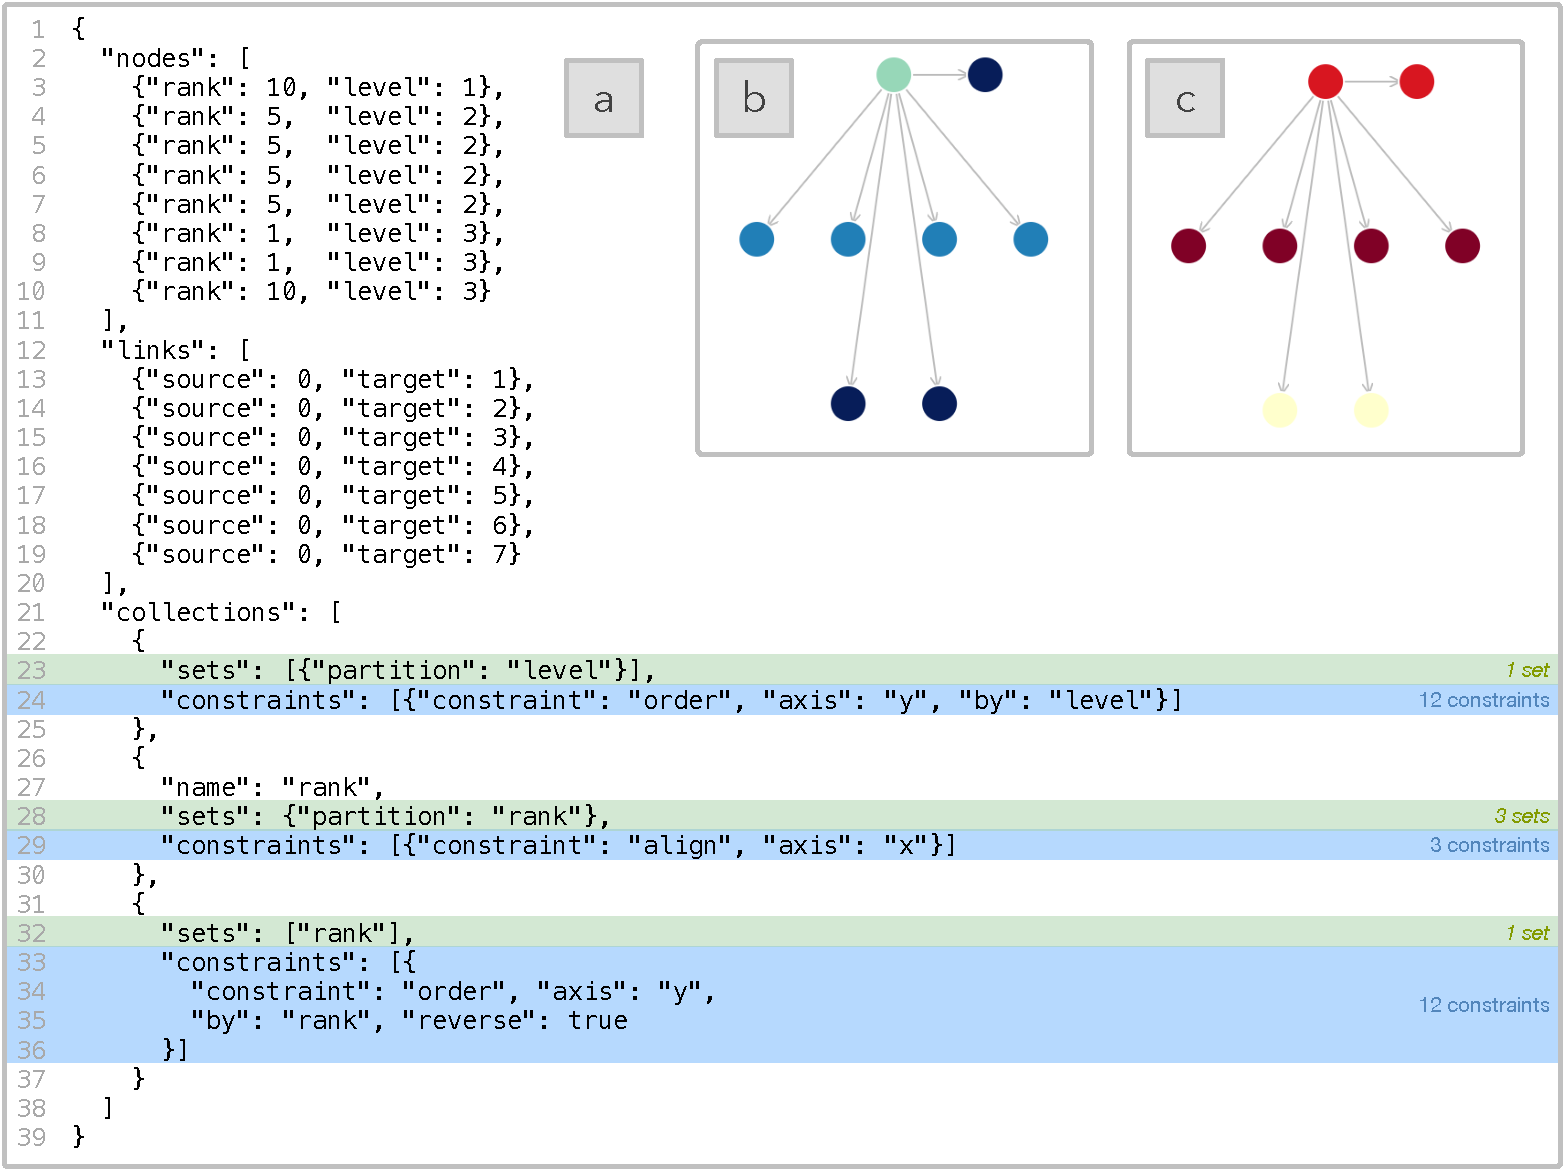
\includegraphics[width=\columnwidth]{figures/contradiction-example.pdf}
    {\caption{\label{fig:contradiction-example}
    (a) The full \projectname\ specification for a small graph with eight nodes. (b) Nodes are aligned based on their \texttt{rank}, and colored based on their \texttt{level}. Two constraints are applied to order the nodes, once by \texttt{level} and once by \texttt{rank}, which produces a contradiction. (c) Nodes are colored based on the amount of error for constraints that are invalid.
    }}
    \vspace{-20px}
  \end{figure}
}

%%%%%%%%%%%%%%%%%%%%%%%%%%%%%%%%%%
%%%%%%%%% Demonstration %%%%%%%%%%
%%%%%%%%%%%%%%%%%%%%%%%%%%%%%%%%%%

\newcommand{\krugerLayout}{
  \begin{figure}[t!]
    \centering
    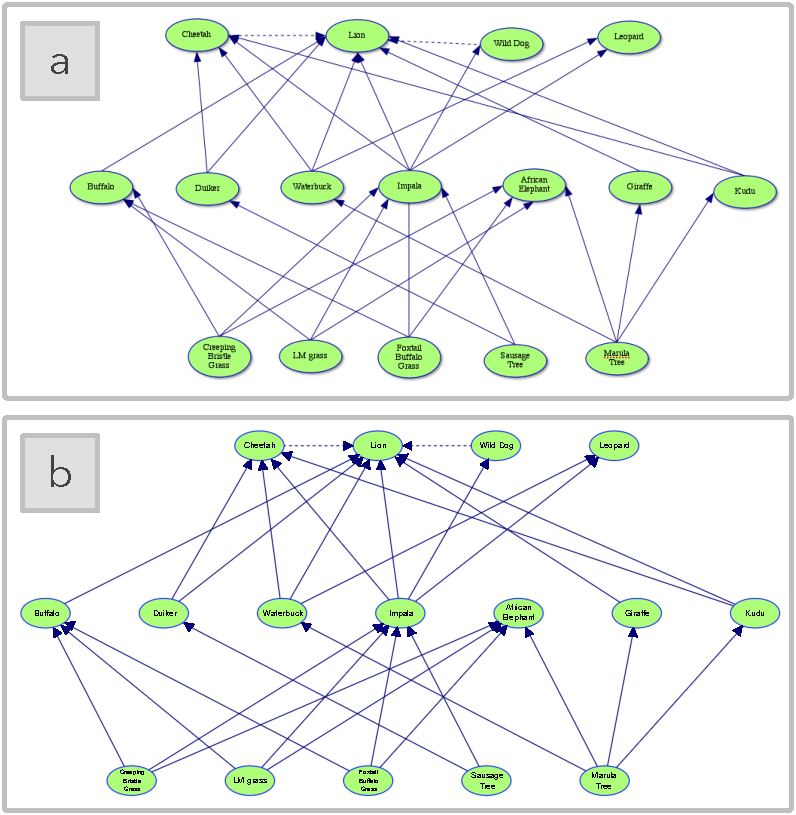
\includegraphics[width=0.81\columnwidth]{figures/kruger-layout.pdf}
    {\caption{\label{fig:kruger-layout}
    The layout for a small subset of the food web for Kruger National Park from (a) their website \orange{citation} as compared to (b) our layout using \projectname.}}
    \vspace{-20px}
  \end{figure}
}

\newcommand{\serengetiLayout}{
  \begin{figure*}[t]
    \centering
    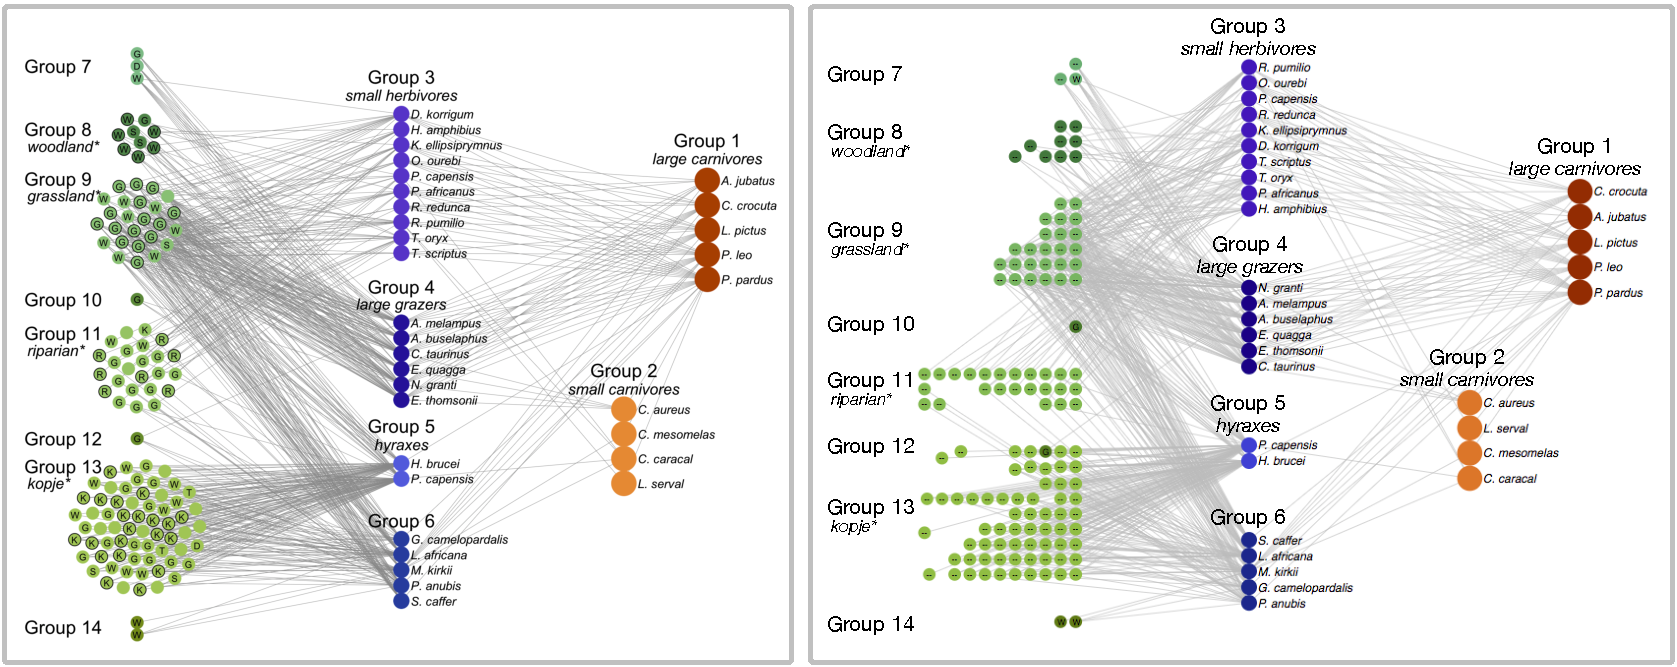
\includegraphics[width=\textwidth]{figures/serengeti-layout.pdf}
    \vspace{-20px}
    {\caption{\label{fig:serengeti-layout}
    The layout for the Serengeti food web using our constraint language, as compared to Baskerville et al. \cite{baskerville2011spatial}. \todo{retake photos on retina screen} \todo{label the two sides of the figure a/b}}}
  \end{figure*}
}

\newcommand{\serengetiSpec}{
  \begin{figure}[t]
    \centering
    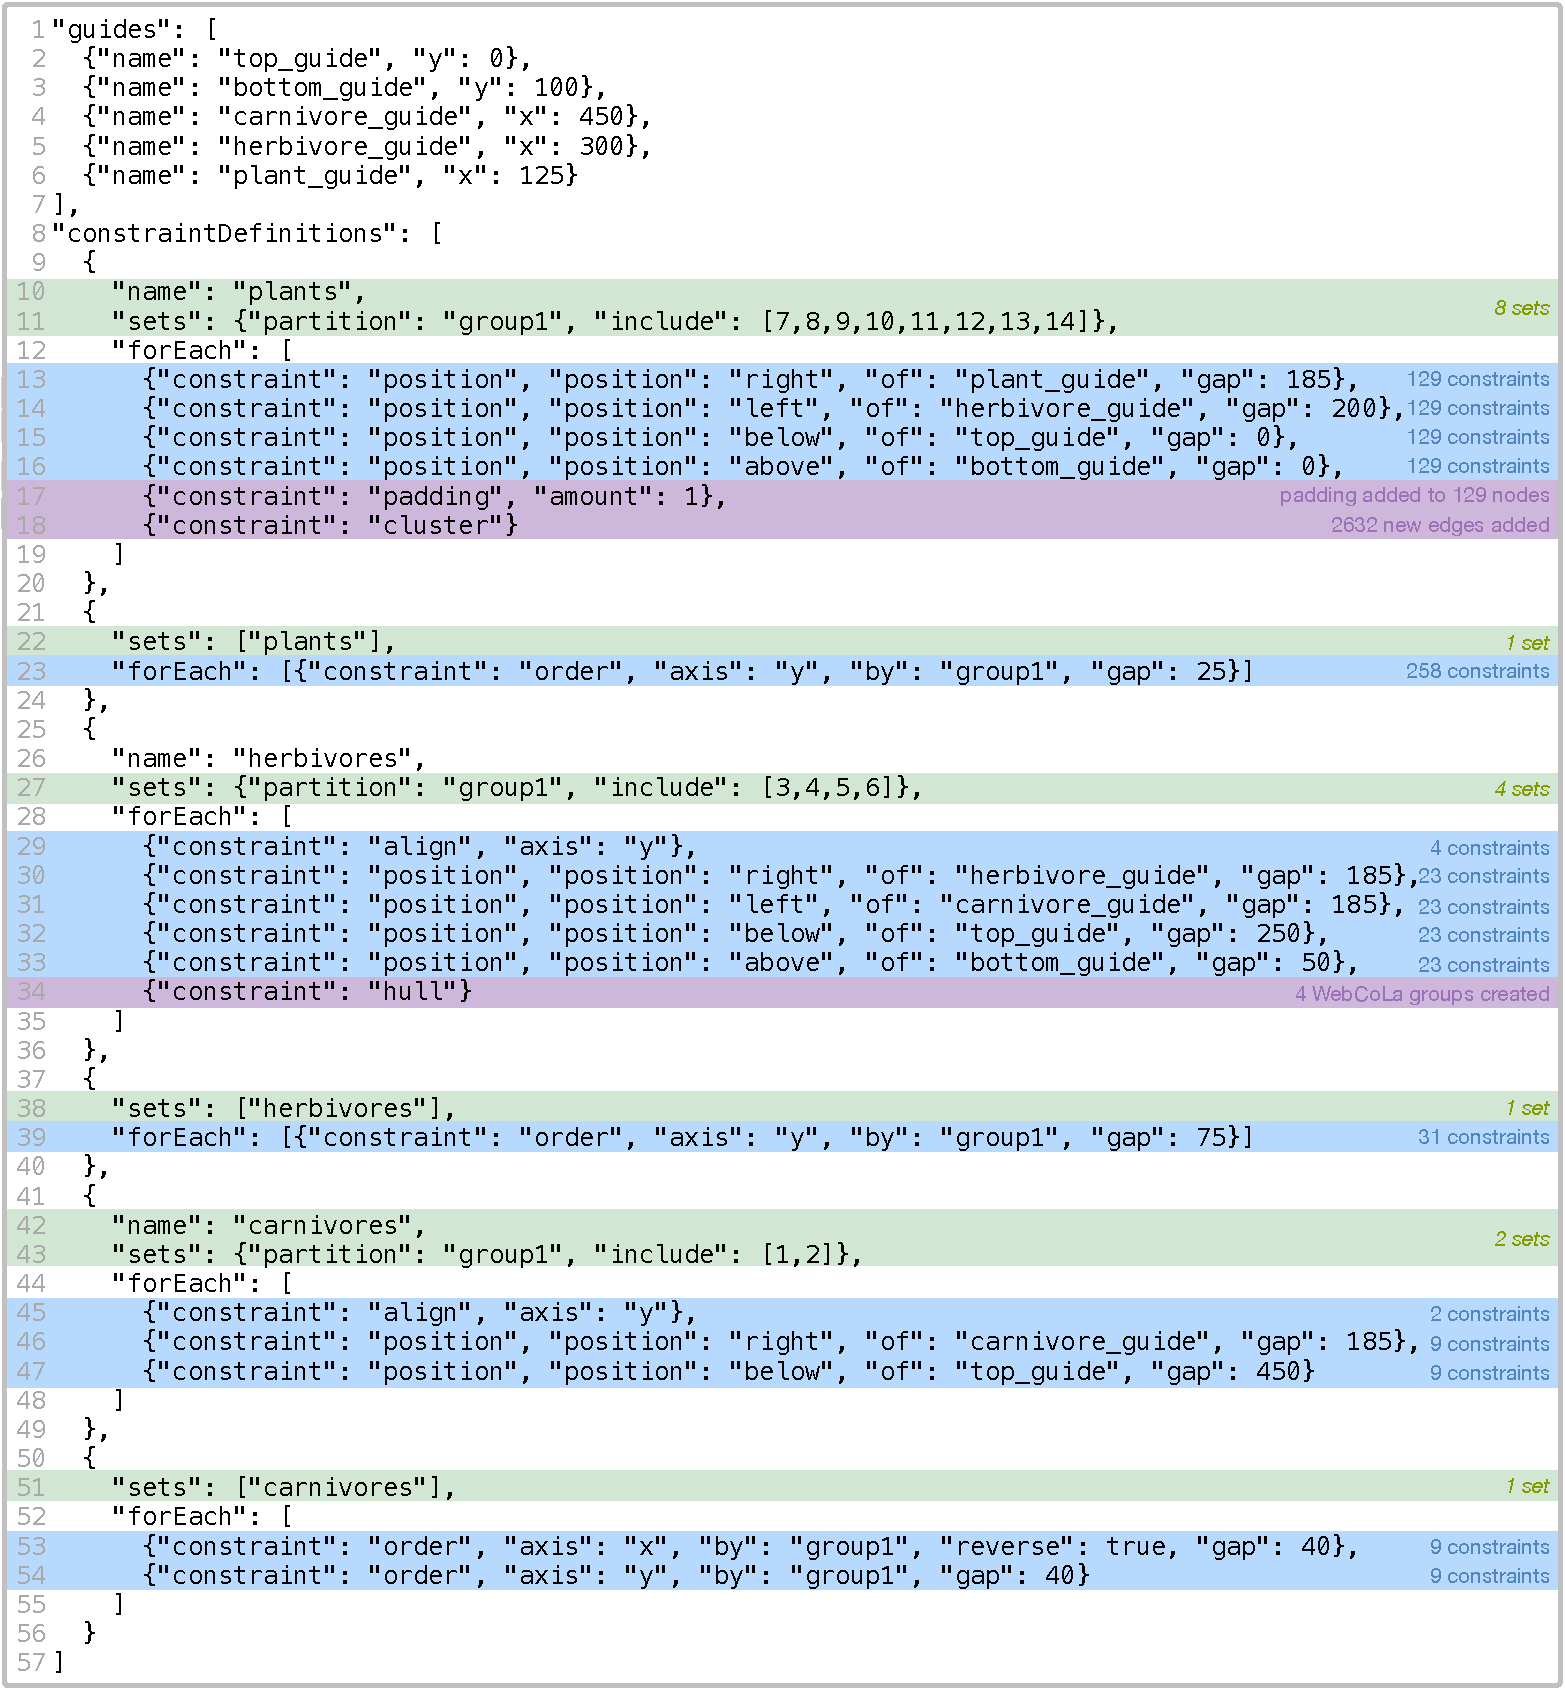
\includegraphics[width=\columnwidth]{figures/serengeti-spec.pdf}
    \vspace{-20px}
    {\caption{\label{fig:serengeti-spec}
    The \projectname~specification for the Serengeti food web shown in Figure~\ref{fig:serengeti-layout}. The code is annotated with the number of sets produced, the number of edges added, and the number of WebCoLa constraints generated for the final layout.}}
  \end{figure}
}

\newcommand{\syphilisLayout}{
  \begin{figure*}[t]
    \centering
    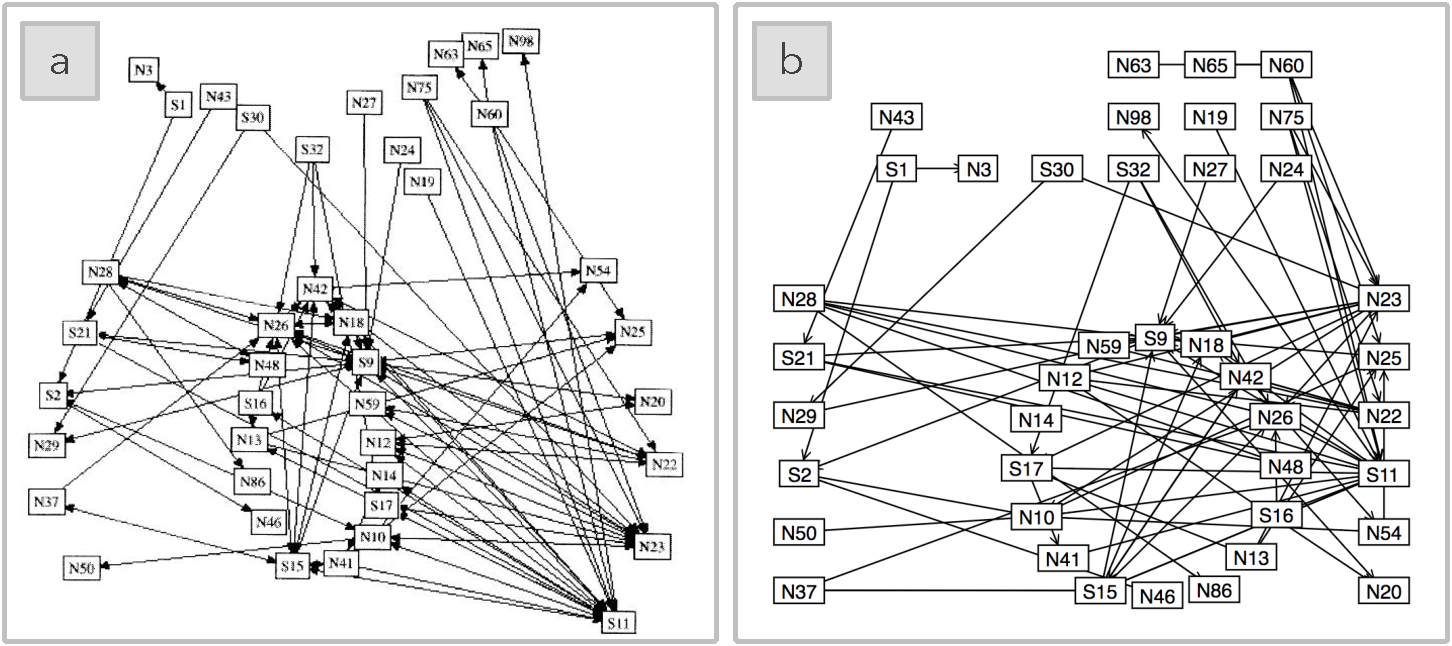
\includegraphics[width=\textwidth]{figures/syphilis-layout.pdf}
    \vspace{-20px}
    {\caption{\label{fig:syphilis-layout}
    The layout for the syphilis social network from (a) Rothenberg et al. \cite{rothenberg1998using} as compared to (b) the \projectname~layout. \todo{add some padding on the layout of the aligned men}}}
  \end{figure*}
}

\newcommand{\syphilisSpec}{
  \begin{figure}[t]
    \centering
    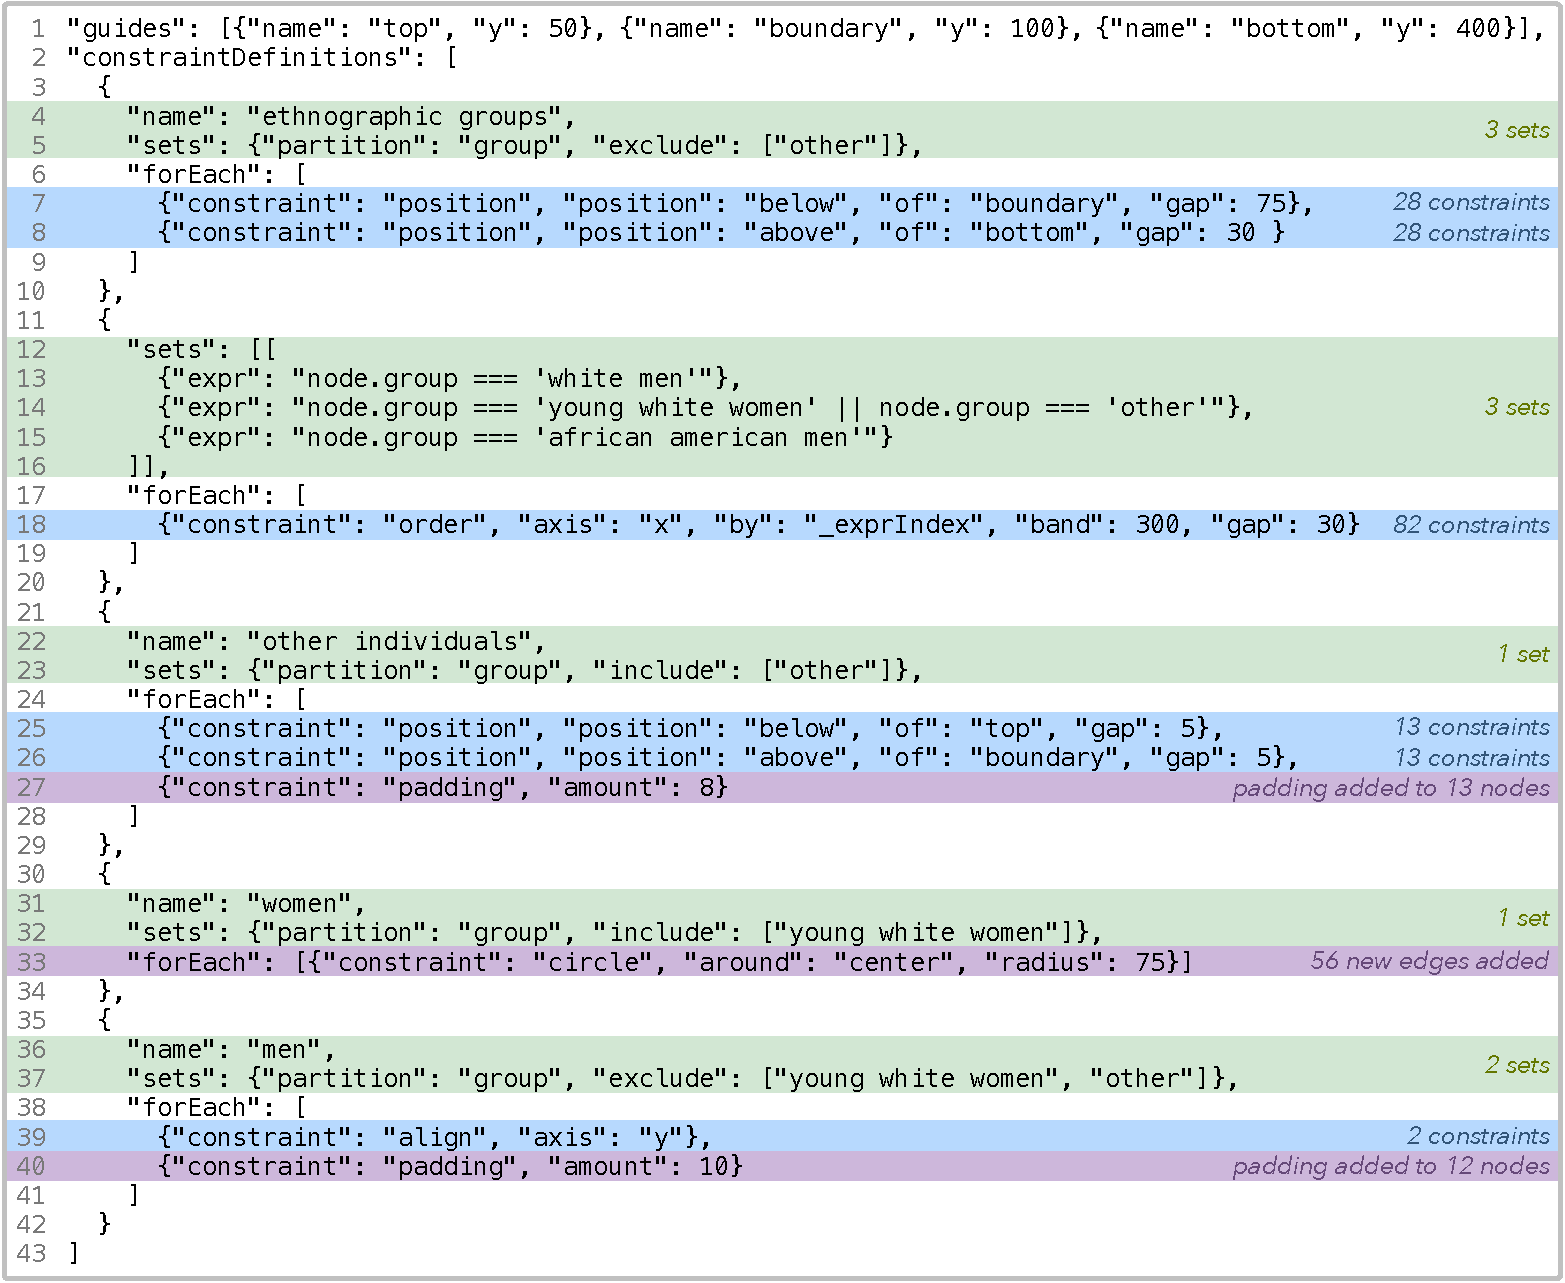
\includegraphics[width=\columnwidth]{figures/syphilis-spec.pdf}
    \vspace{-20px}
    {\caption{\label{fig:syphilis-spec}
    The \projectname~specification for the syphilis social network shown in Figure~\ref{fig:syphilis-layout}. The code is annotated with the number of sets produced, the number of edges added, and the number of WebCoLa constraints generated for the final layout.}}
  \end{figure}
}
\hyphenpenalty=100000

%-------------------------------------------------------------------------
\begin{document}
\maketitle

In our paper, we showed how SetCoLa could be used to recreate Cerebral 
layouts for the TLR4 network. We demonstrate 
the reapplication of a similar SetCoLa specification across networks 
extracted from InnateDB. InnateDB \cite{breuer2012innatedb} is a public 
database containing a large quantity of biological information and is 
integrated with analytic and visualization tools. For example, the database 
is integrated with Cerebral \cite{barsky2008cerebral} to enable visualization 
of properties such as protein interactions or signaling pathways. The 
general specification used for each layout is shown in Figure \ref{fig:specification}.
We selected four networks from InnateDB to recreate with the layout. For 
each one, we apply the same specification and show the result produced with
SetCoLa as compared to the visualization produced by Cerebral.

To demonstrate the reapplication of a SetCoLa specification for similar
graphs in the same domain, we used four examples from InnateDB: 
the TLR4 network~(Figure \ref{fig:tlr4Innate}, \cite{innatedb:tlr4}), 
the DDX58 network~(Figure \ref{fig:ddx58Innate}, \cite{innatedb:ddx58}), 
the NOD-like signaling pathway~(Figure \ref{fig:nodInnate}, \cite{innatedb:nod}), 
and the MAPK1 network~(Figure \ref{fig:mapk1Innate}, \cite{innatedb:mapk1}).
The full specification and data for each example is included in the other 
supplementary materials, along with the other specifications from the paper.
For each figure, we added custom labels to match the labels produced by
Cerebral in order to facilitate the comparison between the two layouts.
These examples show that that layout can easily be reapplied across
different graphs using the same SetCoLa specification. 

While the SetCoLa specification works well for the TLR4 network, DDX58 
network, and NOD-like signaling pathway, the specification produces an 
undesirable result for the MAPK1 network (Figure \ref{fig:mapk1Innate}b). 
This graph produces a much more flattened version of the network because 
it has over twice the number of nodes as the other networks (e.g., 240 
nodes as compared to about 100 in the smaller networks). In this case, 
the constants used in the specification are not particularly ideal for 
the larger network. Future work should explore better techniques for 
applying spacing relative to graph properties rather than constant 
values. An improved version of the MAPK1 network (with reduced spacing 
on the nodes in the ``Nucleus'' layer) is shown in Figure \ref{fig:mapk1Innate}c.
One of the other main differences between the SetCoLa and Cerebral specifications is
the rendering style for the links, which uses a bundled routing style in Cerebral.
Such a rendering style could be added to SetCoLa in the future to achieve this effect.
\\
\\

\begin{figure}[t]
  \centering
  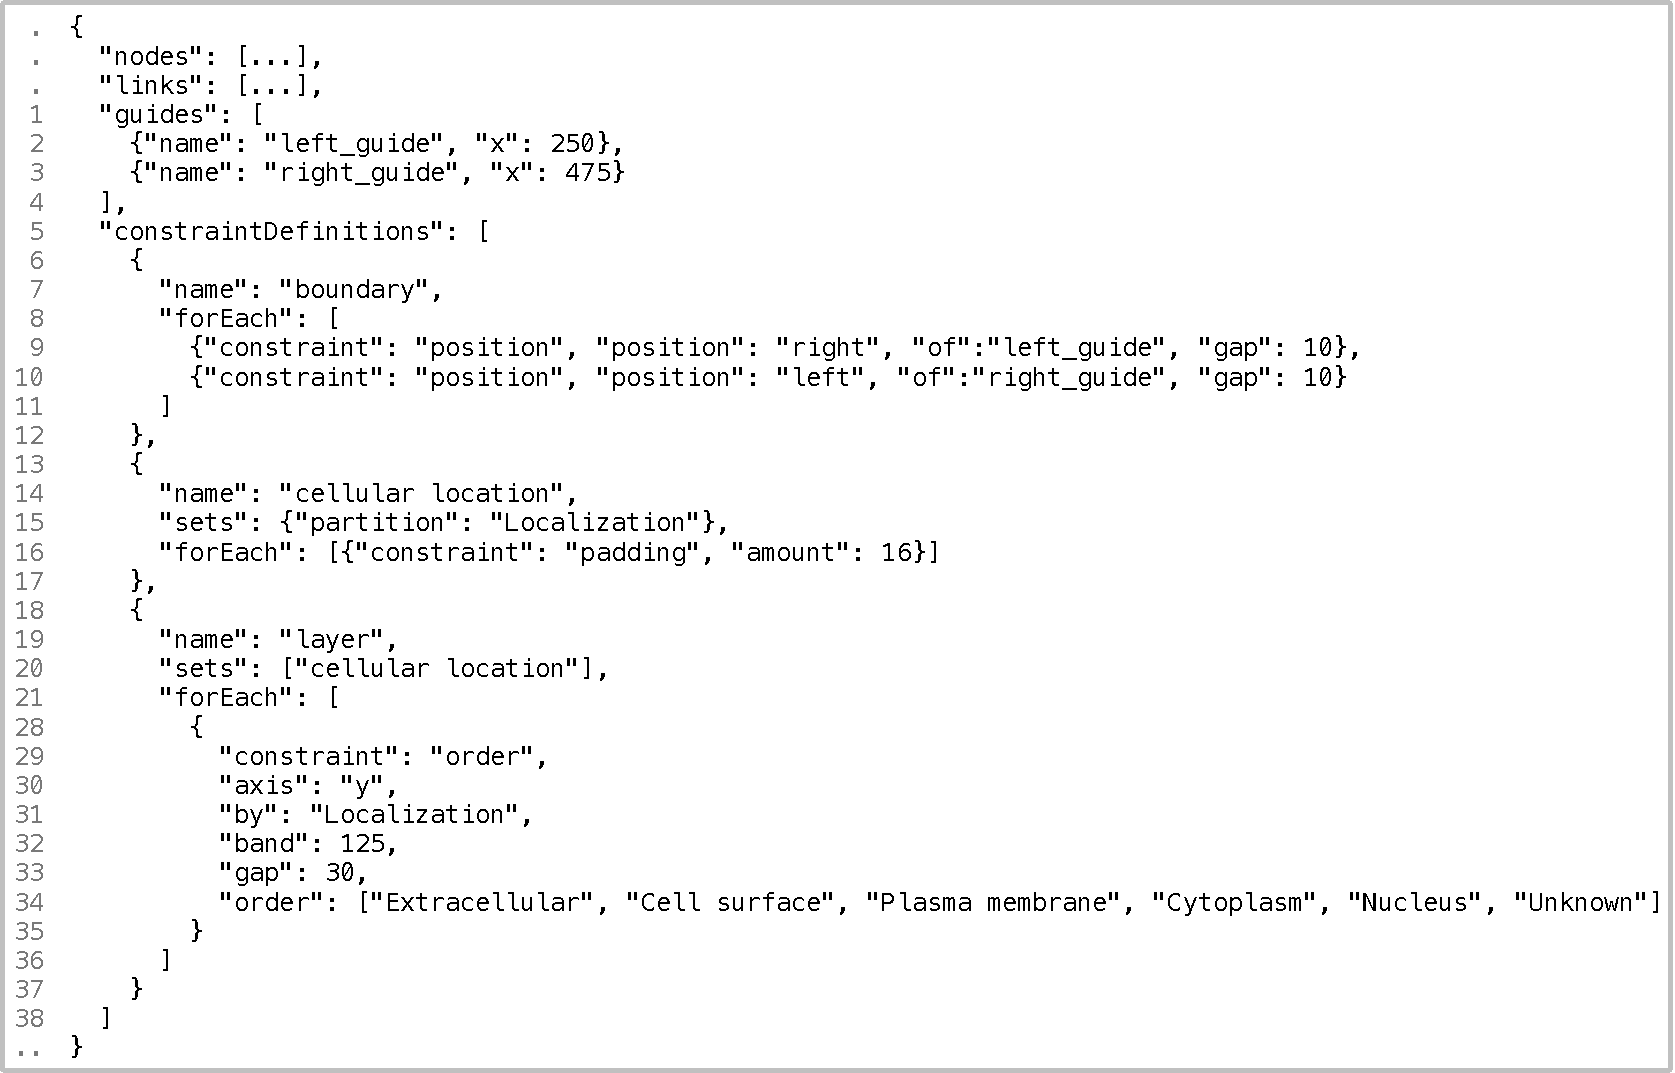
\includegraphics[width=\columnwidth]{figures/innatedb-specification.pdf}
  \vspace{-11px} {\caption{\label{fig:specification} 
    The specification reapplied across four biological networks: 
    TLR4 interaction network (Figure \ref{fig:tlr4Innate}),
    DDX58 interaction network (Figure \ref{fig:ddx58Innate}),
    the NOD-like signaling pathway (Figure \ref{fig:nodInnate}),
    and MAPK1 interaction network (Figure \ref{fig:mapk1Innate}).
  }}
\end{figure}

\begin{figure*}[t]
  \centering
  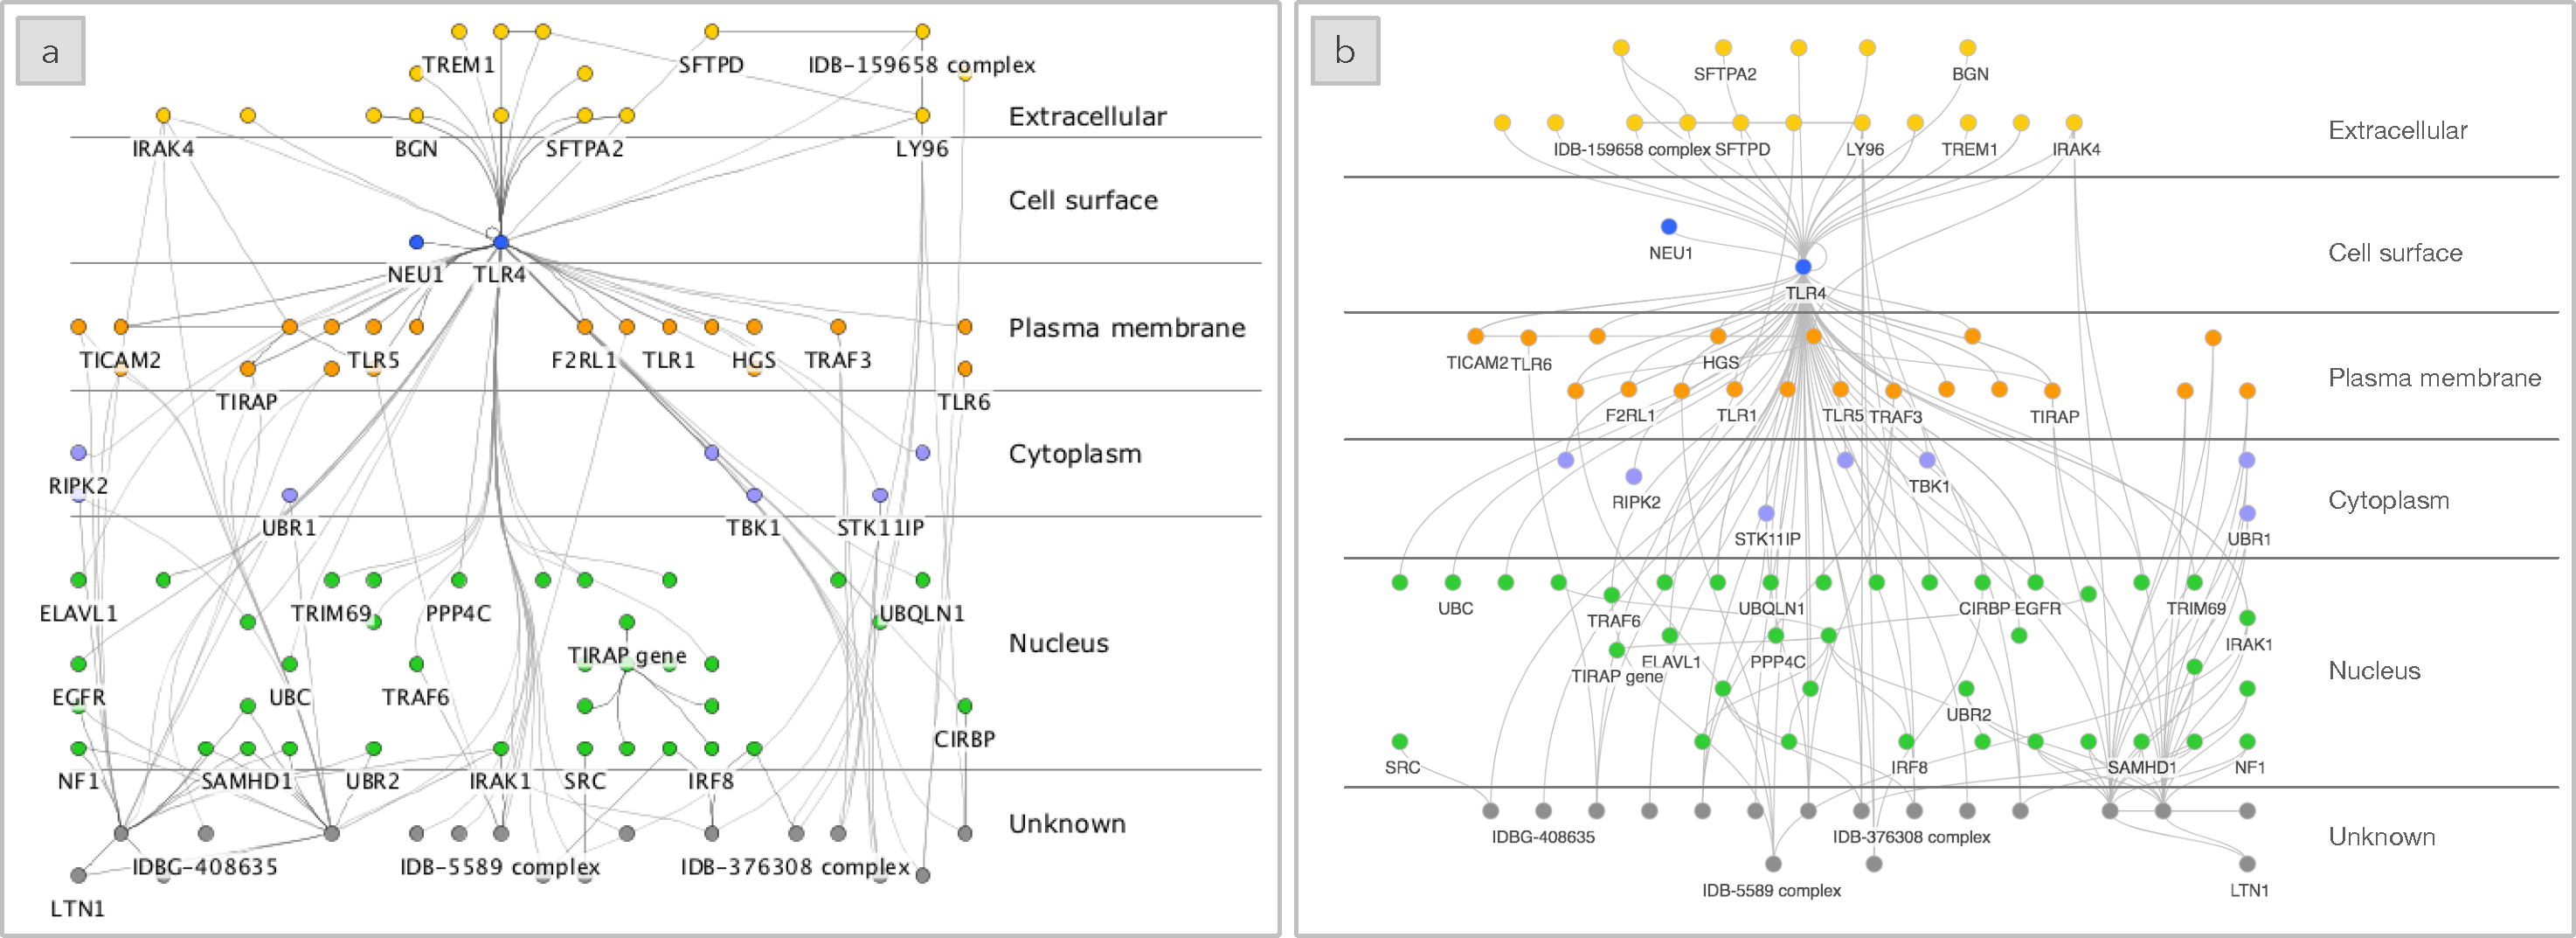
\includegraphics[width=\textwidth]{figures/innatedb-tlr4.pdf}
  \vspace{-15px} {\caption{\label{fig:tlr4Innate} 
    The layout for the TLR4 biological system produced using 
    (a) the Cerebral visualization from InnateDB~\cite{innatedb:tlr4}
    as compared to (b) SetCoLa. The layers correspond to the 
    location of the biomolecule within a cell.
  }}
  \vspace{-10px}
\end{figure*}

\begin{figure*}[t]
  \centering
  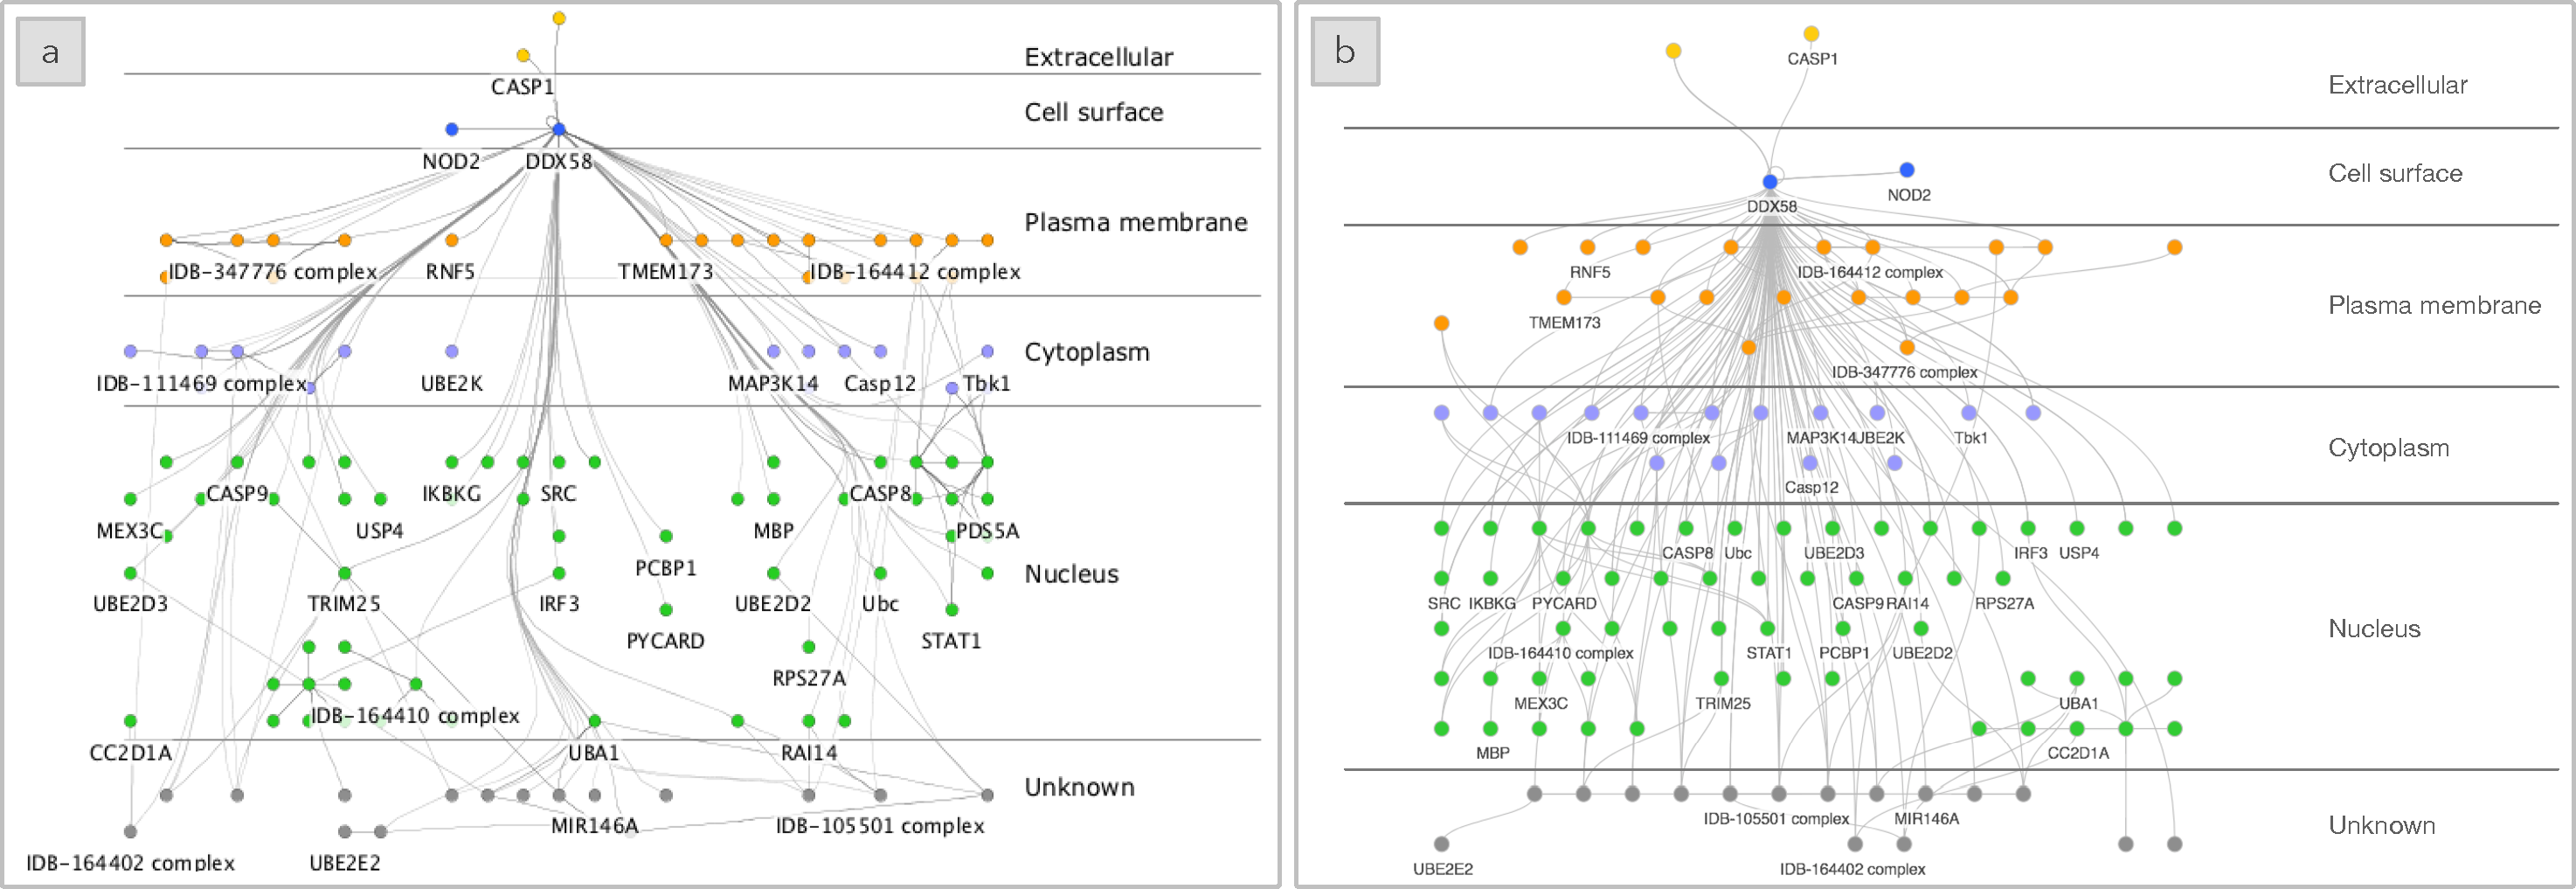
\includegraphics[width=\textwidth]{figures/innatedb-ddx58.pdf}
  \vspace{-15px} {\caption{\label{fig:ddx58Innate} 
    The layout for the DDX58 biological system produced using 
    (a) the Cerebral visualization from InnateDB~\cite{innatedb:ddx58}
    as compared to (b) SetCoLa. The layers correspond to the 
    location of the biomolecule within a cell.
  }}
  \vspace{-10px}
\end{figure*}

\begin{figure*}[t]
  \centering
  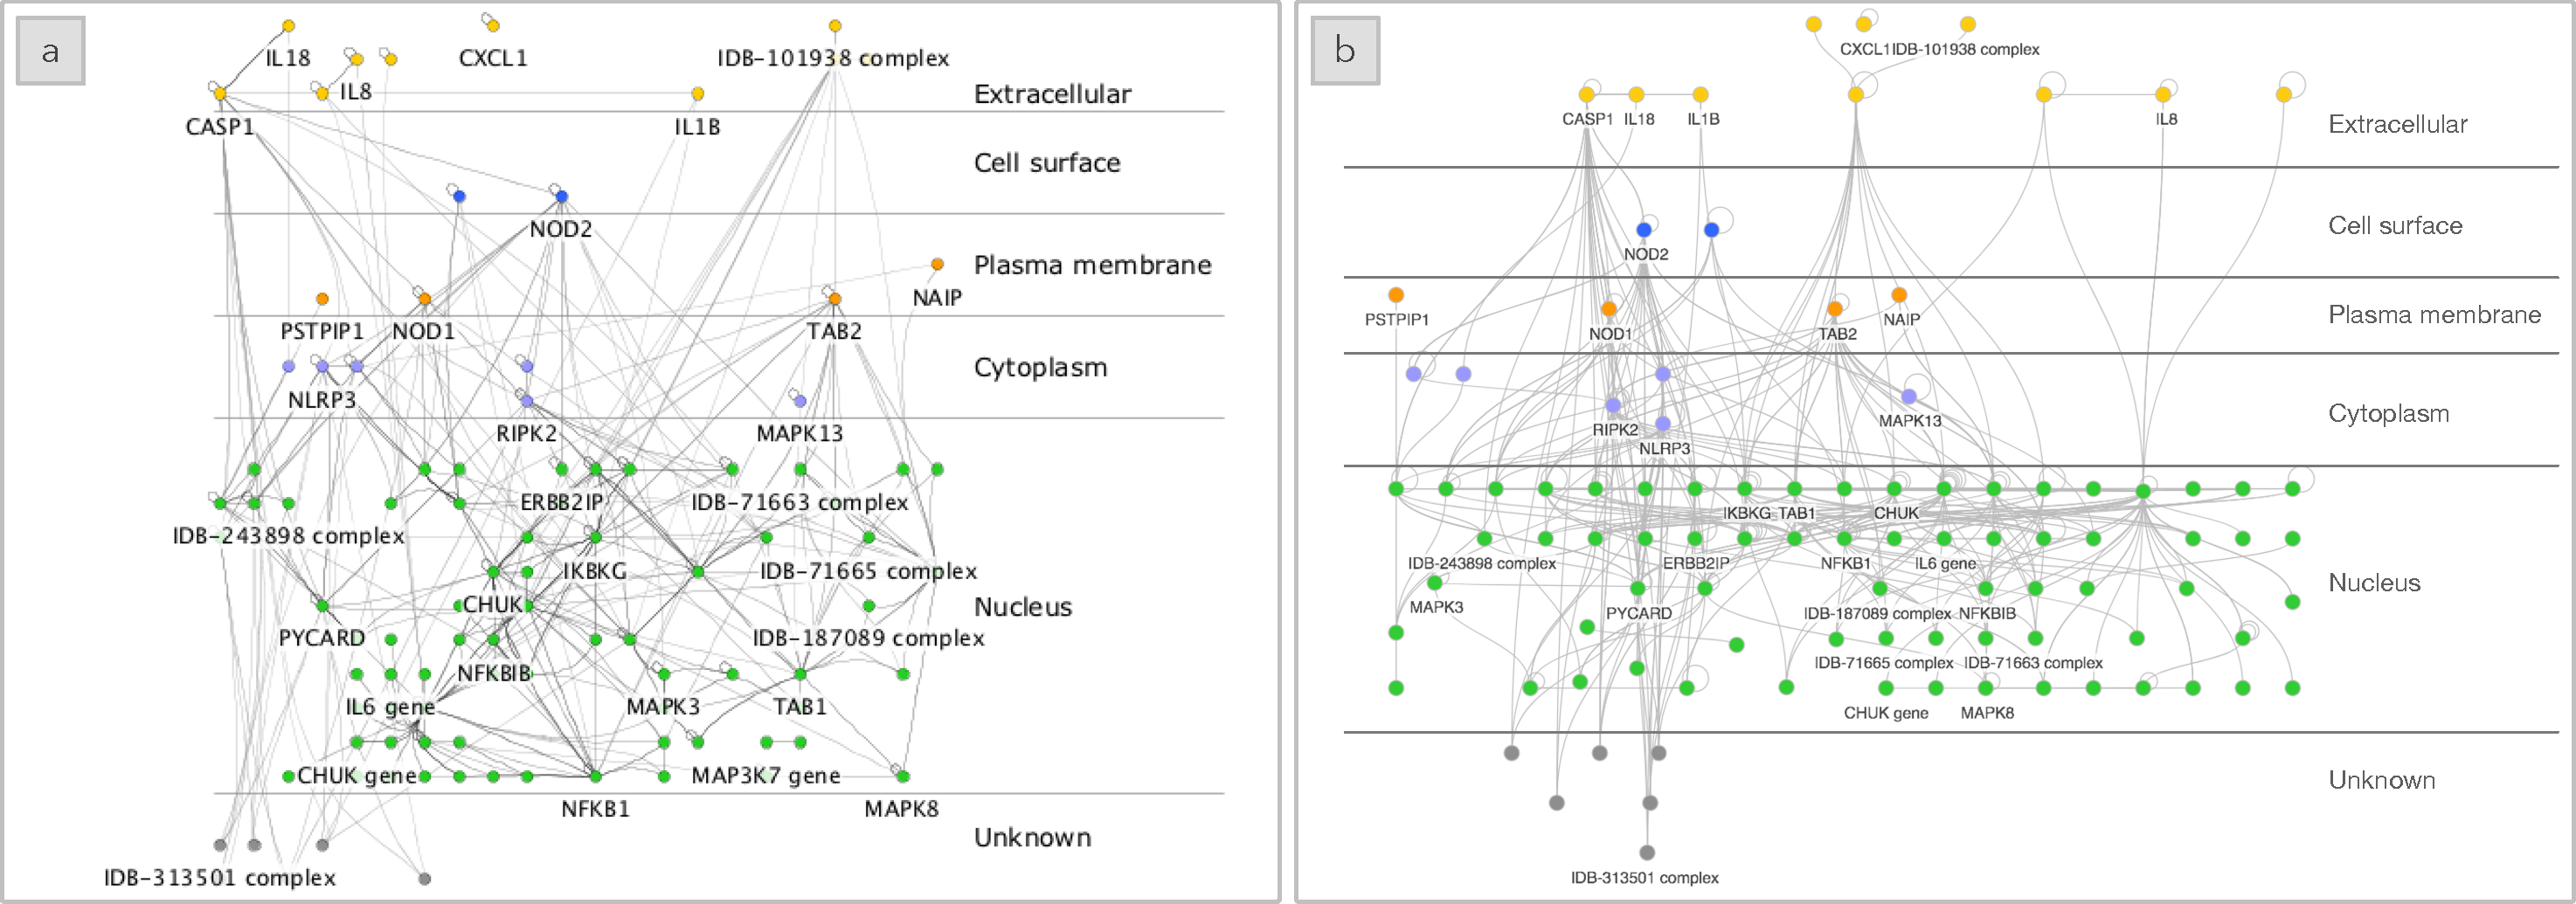
\includegraphics[width=\textwidth]{figures/innatedb-nod.pdf}
  \vspace{-15px} {\caption{\label{fig:nodInnate} 
    The layout for the NOD-like signaling pathway produced using 
    (a) the Cerebral visualization from InnateDB~\cite{innatedb:nod}
    as compared to (b) SetCoLa. The layers correspond to the 
    location of the biomolecule within a cell.
  }}
  \vspace{-10px}
\end{figure*}

\begin{figure*}[t]
  \centering
  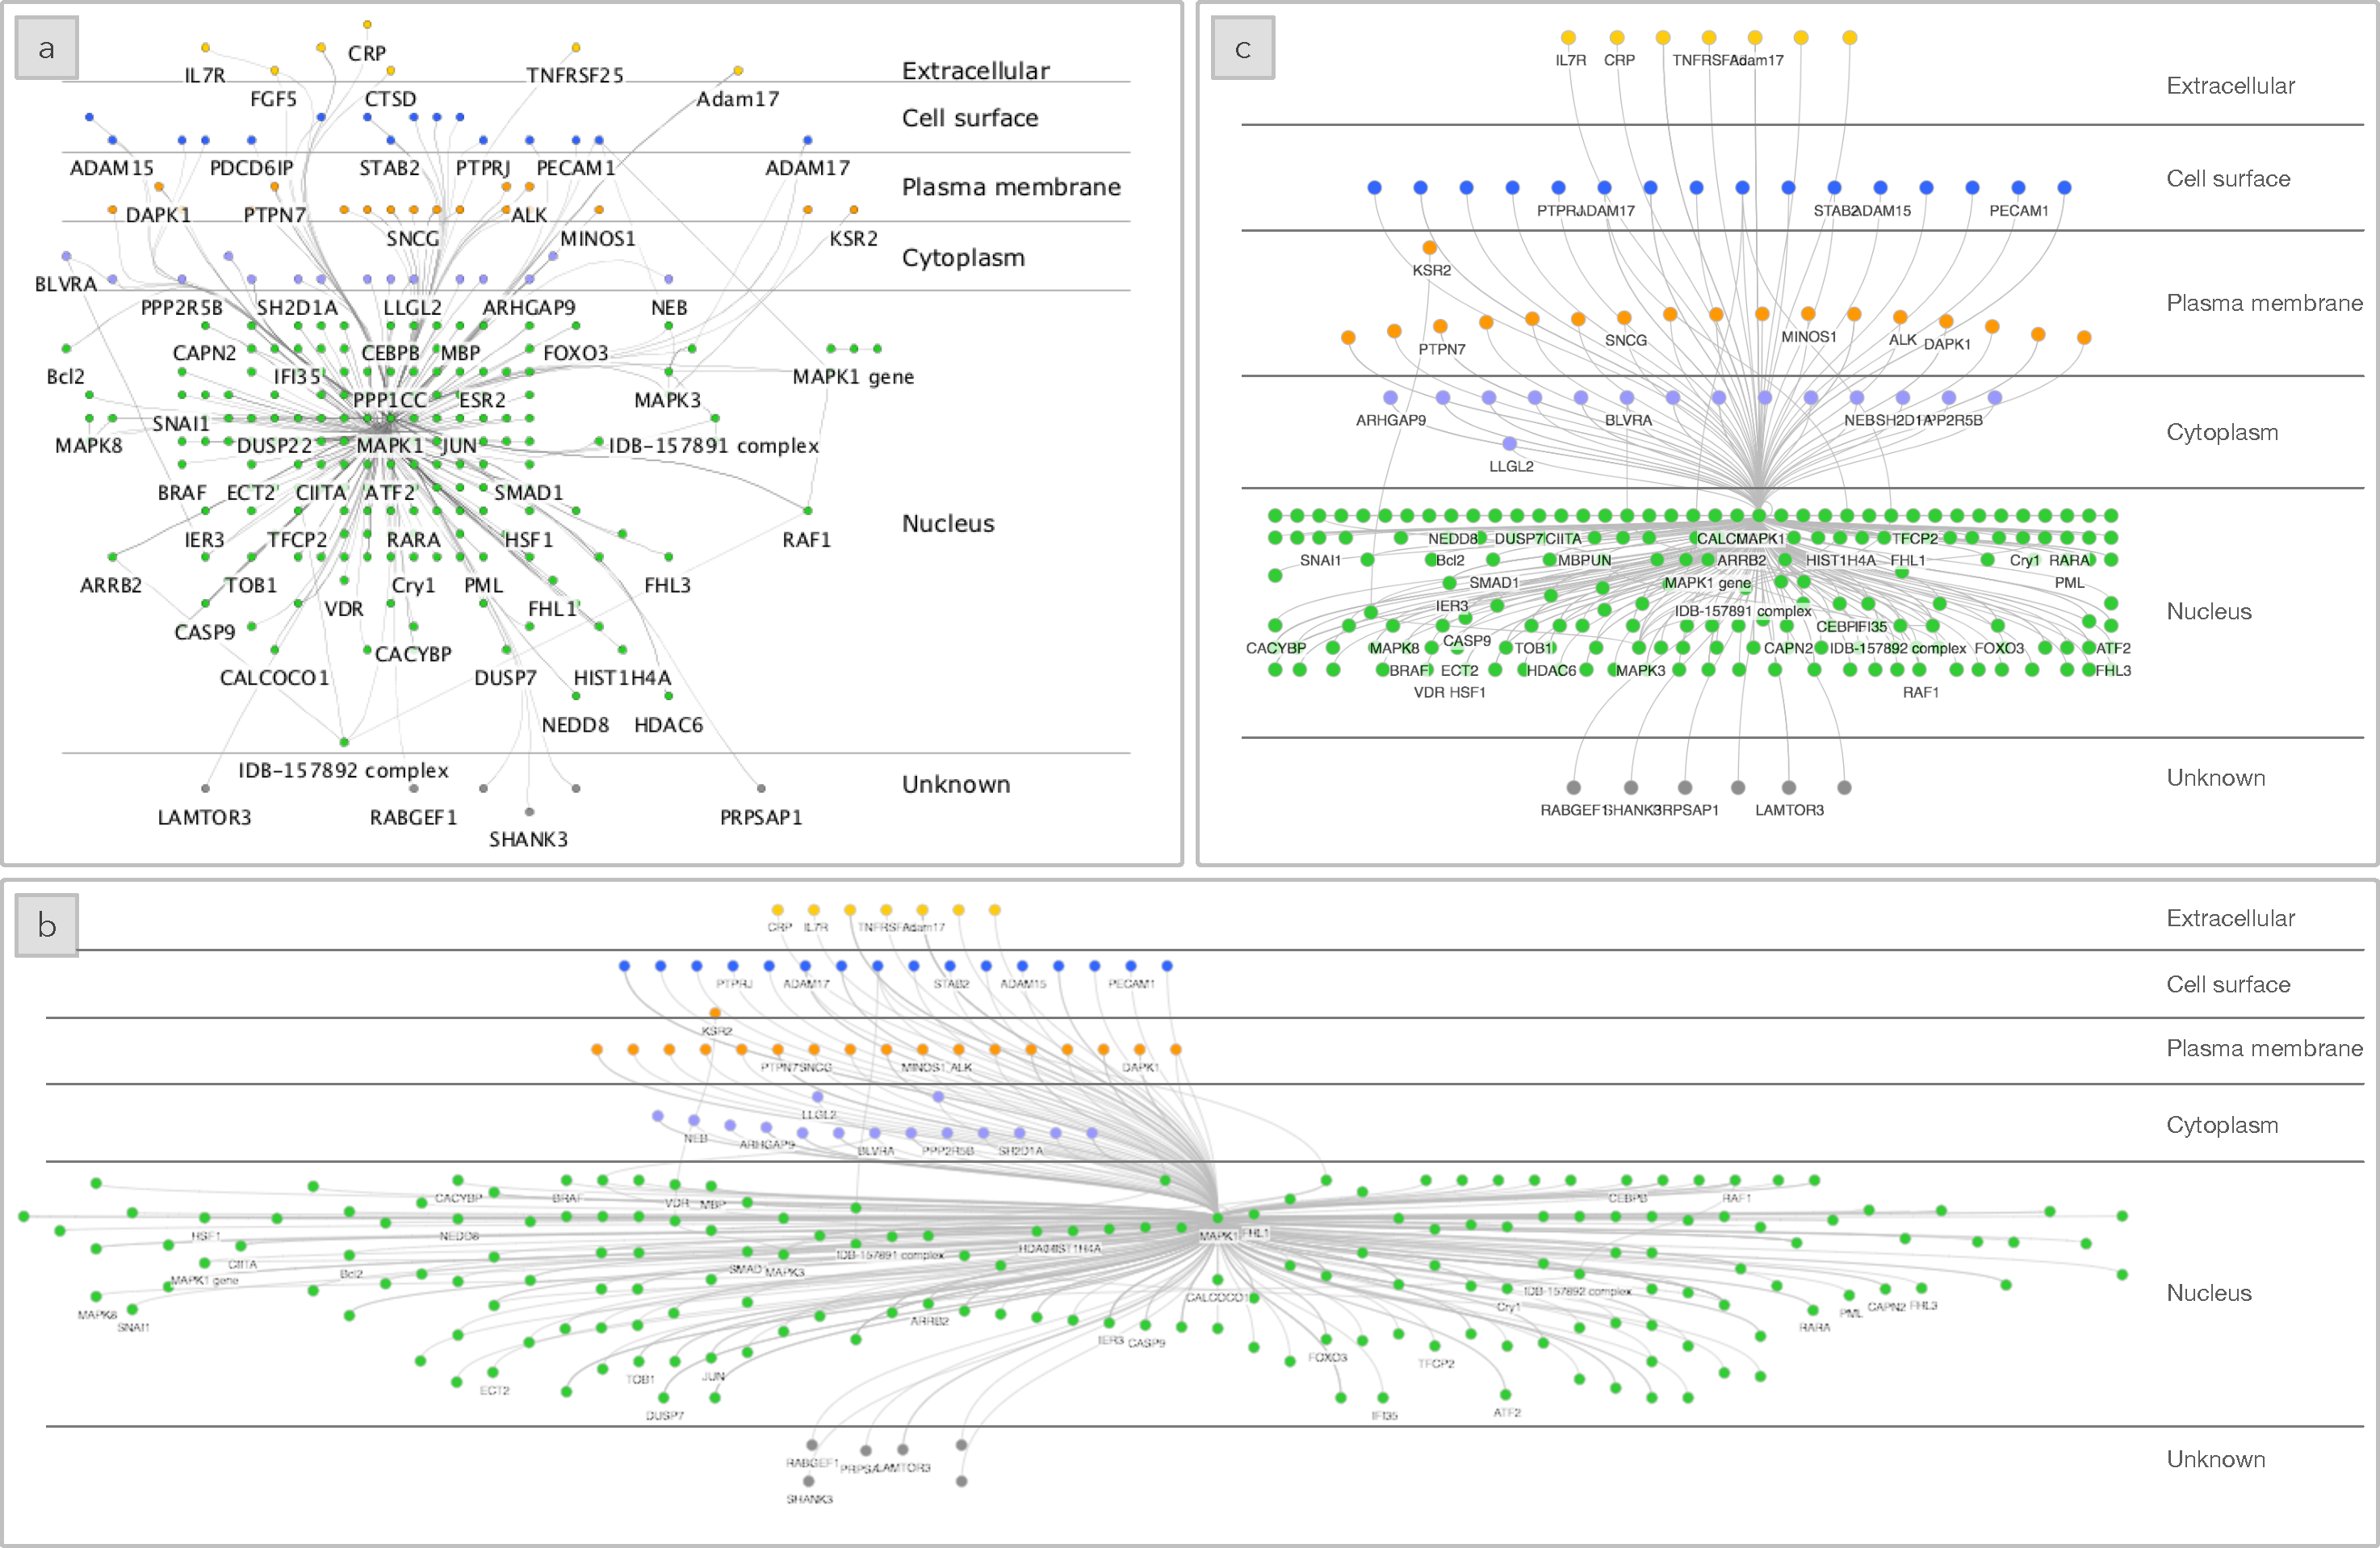
\includegraphics[width=\textwidth]{figures/innatedb-mapk1.pdf}
  \vspace{-15px} {\caption{\label{fig:mapk1Innate} 
    The layout for the MAPK1 biological system produced using 
    (a) the Cerebral visualization from InnateDB~\cite{innatedb:mapk1}
    as compared to (b) SetCoLa. The layers correspond to the 
    location of the biomolecule within a cell. The excessive spacing
    and constraints on the size of each layer produces an undesirable
    layout for the larger graph as compared to the smaller alternatives
    (Figures \ref{fig:tlr4Innate}, \ref{fig:ddx58Innate}, \ref{fig:nodInnate}).
    (c) By adding an additional constraint to reduce the spacing, we can
    achieve a more desirable layout for this graph.
  }}
\end{figure*}

%-------------------------------------------------------------------------

%\bibliographystyle{eg-alpha}
\bibliographystyle{eg-alpha-doi}
\bibliography{supplemental-references}

\end{document}
